\documentclass[11pt]{amsart}
\usepackage[a4paper,margin=1in]{geometry}
\usepackage{amssymb,amsmath}
\usepackage{tikz}
\usepackage[font=small,labelfont=bf]{caption}
\usepackage[hidelinks]{hyperref}

\colorlet{copper}{orange!75!black}
\colorlet{inkmuted}{black!60}

\newtheorem{theorem}{Theorem}
\newtheorem{lemma}[theorem]{Lemma}
\theoremstyle{remark}
\newtheorem{remark}[theorem]{Remark}

\title{Critical Random Discs Cover the Disc}
\author{Vamshi Jandhyala}
\address{London, United Kingdom}
\email{vamshi.jandhyala@gmail.com}

\begin{document}

\begin{abstract}
Place discs of areas $\pi,\pi/2,\pi/3,\dots$ with independent centres uniform in the closed unit disc. A MathOverflow question asks whether they cover the unit disc almost surely. This is the critical case: with areas $c\pi/n$ the uncovered set has dimension $2(1-c)$, and at $c=1$ known sufficient conditions do not decide it. We show that the answer is yes, assuming a recent exact criterion of Zhou for random ball coverings of tori, which has not yet been refereed. The interior reduces to Zhou's criterion by a measure-preserving localisation, and the criterion holds because two unit discs at distance $s$ overlap in area at least $\pi(1-s)$. The boundary circle is a critical case of Shepp's theorem with random arc lengths and needs only classical tools. The analytic estimates are checked in Lean.
\end{abstract}

\maketitle

\section{The question}

Let $X_1,X_2,\dots$ be independent and uniform in the closed unit disc $D$, and let $B_n$ be the open disc of radius $r_n=n^{-1/2}$, area $\pi/n$, centred at $X_n$. Is $D$ covered almost surely? A MathOverflow user asked this~\cite{MO}. The total area $\sum\pi/n$ is infinite, and a fixed point is covered infinitely often almost surely, since it lies in $B_n$ with probability about $1/n$. The question is whether \emph{every} point is covered.

The areas are exactly critical. With areas $c\pi/n$, the uncovered set of the Poisson version of the model has dimension $2(1-c)$~\cite[Thm.~3.6]{BE}, so the answer is no for $c<1$ and yes for $c>1$, and $c=1$ is the boundary. At the boundary, lower-order terms decide. Biermé and Estrade give a necessary and a sufficient condition for Poisson balls in $\mathbb R^d$ and show that critical intensities can go either way~\cite[Props.~2.4, 2.5]{BE}; for this scale-invariant intensity their sufficient condition fails narrowly (the relevant expression tends to $e^{-3}$ rather than to infinity), so they do not settle it.

Zhou has recently given an exact criterion for balls on a torus~\cite[Thm.~2.1]{Z}. Let $\mathbb T^d=(\mathbb R/\mathbb Z)^d$ with Haar measure $m$, $d\ge2$, let the centres be independent and uniform, the radii $r_1\ge r_2\ge\dots\downarrow0$, and put $u_n(z)=m\bigl(B(0,r_n)\cap B(z,r_n)\bigr)$ and $H(z)=\sum_nu_n(z)$. Then every point is covered infinitely often almost surely if and only if $\int_{\mathbb T^d}e^{H}\,dm=\infty$.

\begin{theorem}\label{thm:main}
Assume Zhou's criterion~\cite[Thm.~2.1]{Z} for $d=2$. Then $D\subset\bigcup_nB_n$ almost surely.
\end{theorem}

Only the interior of $D$ uses Zhou's criterion; the boundary circle is covered almost surely by Shepp's theorem alone (Section~\ref{sec:rim}).

\section{The interior}

\emph{Localisation.} Fix $p$ in the open disc and $\delta>0$ with $B(p,4\delta)\subset D$ and $4\delta<\sqrt\pi/2$. Let $S$ be the square of side $\sqrt\pi$ centred at $p$, a fundamental domain of the torus $T=\mathbb R^2/\sqrt\pi\,\mathbb Z^2$, which has area $\pi$. Since $|D|=|S|=\pi$ there is a measure-preserving bijection $\varphi:D\to S$, up to null sets, that is the identity on $D\cap S$. Then $Y_n=\varphi(X_n)$ are independent and uniform on $T$. Put $K=\overline B(p,\delta)$. Once $r_n<\delta$, a torus ball $B(Y_n,r_n)$ that meets $K$ has $Y_n\in B(p,2\delta)\subset D\cap S$, so $Y_n=X_n$ and the torus ball is $B_n$. Hence if the balls $B(Y_n,r_n)$ cover every point of $T$ infinitely often, then $K\subset\bigcup_nB_n$. Countably many such $K$ cover the open disc.

\emph{The criterion.} Scaling $T$ to $(\mathbb R/\mathbb Z)^2$ turns the radii into $\rho_n=(\pi n)^{-1/2}$, with $m(B(0,\rho_n))=1/n$, and
\[
u_n(z)=\frac1n\,\psi\Bigl(\frac{|z|}{\rho_n}\Bigr),
\]
where $\pi\psi(s)$ is the area of the lens in which two unit discs at distance $s$ overlap. The lens contains the disc of radius $1-s/2$ about the midpoint of the centres (Figure~\ref{fig:lens}): a point within $1-s/2$ of the midpoint is within $1-s/2+s/2=1$ of each centre. So
\begin{equation}\label{eq:lens}
\psi(s)\ \ge\ \Bigl(1-\frac s2\Bigr)^2\ \ge\ 1-s\qquad(0\le s\le2).
\end{equation}
For small $t=|z|$ let $N=\lfloor1/(\pi t^2)\rfloor$, so that $|z|/\rho_n=t\sqrt{\pi n}\le1$ for $n\le N$. Dropping the terms with $n>N$, which are nonnegative, and using $\sum_{n\le N}1/n\ge\log(N+1)$ and $\sum_{n\le N}n^{-1/2}\le2\sqrt N$,
\[
H(z)\ \ge\ \sum_{n=1}^N\frac1n\bigl(1-t\sqrt{\pi n}\bigr)\ \ge\ \log(N+1)-2t\sqrt{\pi N}\ \ge\ 2\log\frac1t-\log\pi-2 .
\]
So $e^{H(z)}\ge c\,|z|^{-2}$ near $0$, and $\int e^H\,dm\ge c\int_0^{t_0}t^{-2}\,2\pi t\,dt=\infty$. By Zhou's criterion the torus is covered infinitely often almost surely, and by the localisation the open disc is covered.

\begin{figure}[ht]
\centering
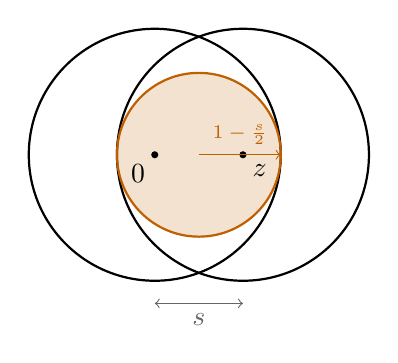
\begin{tikzpicture}[scale=1.6]
  \fill[copper!18] (0.35,0) circle (0.65);
  \draw[thick] (0,0) circle (1);
  \draw[thick] (0.7,0) circle (1);
  \draw[copper,thick] (0.35,0) circle (0.65);
  \fill (0,0) circle (0.8pt) node[below left] {$0$};
  \fill (0.7,0) circle (0.8pt) node[below right] {$z$};
  \draw[inkmuted,<->] (0,-1.18) -- (0.7,-1.18) node[midway,below] {$s$};
  \draw[copper,->] (0.35,0) -- (1.0,0) node[midway,above,font=\scriptsize] {$1-\frac s2$};
\end{tikzpicture}
\caption{Two unit discs at distance $s$ overlap in a lens that contains the disc of radius $1-s/2$ about the midpoint, so the lens has area at least $\pi(1-s/2)^2\ge\pi(1-s)$. This is the only estimate the interior needs.}
\label{fig:lens}
\end{figure}

\section{The rim}\label{sec:rim}

For $|X_n|=\rho$, the set $B_n\cap S^1$ is empty if $\rho\le1-r_n$ and otherwise an arc centred at the angle $\arg X_n$. Let $\ell_n$ be its length as a fraction of the circle. Since $\arg X_n$ is uniform and independent of $|X_n|$, conditionally on the lengths $(\ell_n)$ the arcs are independent with uniform positions. Shepp's theorem~\cite{S},~\cite[Ch.~11]{K} then says that the circle is covered almost surely if and only if
\begin{equation}\label{eq:shepp}
\int_0^1e^{F(t)}\,dt=\infty,\qquad F(t)=\sum_n(\ell_n-t)^+ .
\end{equation}
This is Shepp's series $\sum_NN^{-2}e^{\ell_1+\dots+\ell_N}=\infty$ for decreasing lengths, rewritten by summation by parts~\cite[\S2, eq.~(3)]{Z}; the integral form is symmetric in the $\ell_n$, so their order and the empty arcs do not matter, and finitely many arcs change $F$ by a bounded amount. We show that~\eqref{eq:shepp} holds almost surely.

\emph{The mean.} By Fubini, $\mathbb E\,\ell_n=|B(q,r_n)\cap D|/\pi$ for any $q\in S^1$. The disc $B(q,r)$ contains the half-disc on the inner side of the tangent line at $q$, except for the sliver between that line and the circle, whose area is at most $\int_{-r}^r\bigl(1-\sqrt{1-x^2}\bigr)\,dx\le\int_{-r}^rx^2\,dx=\frac23r^3$. So $\mathbb E\,\ell_n\ge\frac1{2n}-\frac2{3\pi}n^{-3/2}$. Also $P(\ell_n>0)=P(|X_n|>1-r_n)\le2r_n$, and $(\ell-t)^+\ge\ell-t\,\mathbf 1_{\ell>0}$. Summing over $n\le N=\lfloor t^{-2}\rfloor$,
\[
\mathbb E\,F(t)\ \ge\ \tfrac12\log N-C-2t\sum_{n\le N}n^{-1/2}\ \ge\ \log\tfrac1t-C' .
\]

\emph{Fluctuations.} An arc of chord at most $2r_n$ has $\ell_n\le r_n/2$, so $\mathbb E\,\ell_n^2\le\frac{r_n^2}4\cdot2r_n\le n^{-3/2}$, which is summable; hence $G_0=\sum_n(\ell_n-\mathbb E\ell_n)$ converges almost surely, by Kolmogorov's two-series theorem. Since $(\ell-t)^+=\ell-\min(\ell,t)$,
\[
F(t)-\mathbb EF(t)-G_0=-\sum_n\bigl(\min(\ell_n,t)-\mathbb E\min(\ell_n,t)\bigr),
\]
whose variance is at most $\sum_n\mathbb E\min(\ell_n,t)^2\le\sum_n2r_n\min(t,r_n/2)^2\le Ct$. With $t_k=2^{-k}$, Chebyshev's inequality and the Borel-Cantelli lemma give $|F(t_k)-\mathbb EF(t_k)-G_0|\le1$ for all large $k$, almost surely. Since $F$ is nonincreasing,
\[
\int_0^1e^{F}\,dt\ \ge\ \sum_k2^{-k-1}e^{F(t_k)}\ \ge\ \sum_{k\ \text{large}}2^{-k-1}\,2^ke^{-C'-|G_0|-1}=\infty .
\]
So, conditionally on the lengths, Shepp's criterion holds almost surely, and the circle is covered almost surely. Together with the interior this proves Theorem~\ref{thm:main}. \qed

\section{Remarks}

With areas $c\pi/n$ the same two computations give $H=2c\log\frac1t+O(1)$ and $\mathbb EF(t)=c\log\frac1t+O(1)$, so both criteria hold exactly when $c\ge1$: the interior and the rim become critical together, a consequence of the scale invariance of $r_n=n^{-1/2}$ in the plane. Numerically, at $c=1$, $H(t)-2\log\frac1t$ levels off near $-0.42$ and $\mathbb EF(t)-\log\frac1t$ near $-2.72$ for $t$ from $10^{-1}$ to $10^{-3.5}$, while at $c=0.9$ both drift away at the predicted rates.

The interior rests on~\cite{Z}, a single-author preprint of September 2026 that has not been refereed; before it, the case of Euclidean balls in the higher-dimensional Shepp problem was open (Kahane settled homothetic simplices; see the introduction of~\cite{Z}). If Zhou's criterion stands, Theorem~\ref{thm:main} is unconditional. The rim uses only Shepp's theorem.

\section{Verification}

The analytic estimates are formally verified in Lean~4 with Mathlib~\cite{mathlib}: the lens containment and~\eqref{eq:lens}, the lower bound $\sum_{n\le N}\frac1n(1-t\sqrt{\pi n})\ge2\log\frac1t-\log\pi-2$ with the harmonic and square-root sums behind it, the divergence of $\int_0t^{-1}\,dt$, and the sliver inequality $1-\sqrt{1-x^2}\le x^2$. Zhou's criterion, Shepp's theorem, the localisation and the probabilistic estimates of the rim are not formalised. A script evaluates $H(t)-2c\log\frac1t$ and $\mathbb EF(t)-c\log\frac1t$ numerically and checks that they level off for $c=1$ and drift for $c=0.9$. Code and Lean files are at~\cite{repo}.

\section*{Acknowledgments}

The question is due to the MathOverflow user Dan. The argument and the Lean formalisation were developed with Claude (Anthropic). The author is responsible for the content.

\begin{thebibliography}{9}
\bibitem{BE} H.~Biermé and A.~Estrade, \emph{Covering the whole space with Poisson random balls}, ALEA Lat. Am. J. Probab. Math. Stat. 9 (2012), 213--229.
\bibitem{K} J.-P.~Kahane, \emph{Some Random Series of Functions}, 2nd ed., Cambridge University Press, 1985.
\bibitem{mathlib} The mathlib Community, \emph{The Lean mathematical library}, in: Proc.\ 9th ACM SIGPLAN Int.\ Conf.\ on Certified Programs and Proofs (CPP 2020), 367--381.
\bibitem{MO} Dan, \emph{Will a unit disk be completely covered by randomly placed disks of area $\pi,\frac{\pi}{2},\frac{\pi}{3},\dots$ with probability $1$?}, MathOverflow question 458793, \url{https://mathoverflow.net/q/458793}.
\bibitem{S} L.~A.~Shepp, \emph{Covering the circle with random arcs}, Israel J. Math. 11 (1972), 328--345.
\bibitem{Z} Y.~Zhou, \emph{The higher-dimensional Shepp problem: an exact criterion for random ball coverings of tori}, arXiv:2609.02156v1 (2 September 2026).
\bibitem{repo} V.~Jandhyala, code and Lean proofs, \url{https://github.com/jvvk/mathematics/tree/main/critical-discs-cover}.
\end{thebibliography}

\end{document}
